%%%%%%
%
% $Autor: Wings $
% $Datum: 2020-01-18 11:15:45Z $
% $Pfad: WuSt/Skript/Produktspezifikation/powerpoint/ImageProcessing.tex $
% $Version: 4620 $
%
%%%%%%

\chapter{Pin-Belegung des NVIDIA Jetson Nanos}


{\tiny  Quelle: \url{https://www.element14.com/community/community/designcenter/single-board-computers/blog/2019/05/21/nvidia-jetson-nano-developer-kit-pinout-and-diagrams}}

%todo Der Text wird schon an anderer Stelle verwendet.

\section{Introduction}



Der NVIDIA Jetson Nano ist ein kompaktes Board mit einer Größe von ca. 70x45mm und einem großen Kühlkörper. 
Es verfügt über einen sehr leistungsstarken Mikrochip, den NVIDIA Tegra X1, der vier ARM-Anwendungsprozessorkerne sowie 128 Grafikprozessoren (GPU) enthält. GPUs werden nicht nur für Grafikzwecke verwendet, denn es stellt sich heraus, dass einige der heute für Computer interessanten Anwendungen, die mit neuronalen Netzen zu tun haben, mit denen Muster mit immer höherer Genauigkeit erkannt werden können, leichter erstellt werden können und mit zunehmender Anzahl von Recheneinheiten eine bessere Leistung erbringen. Die Vollversion des Tegra X1 (mit doppelt so vielen GPU-Kernen) ist für einige recht unterschiedliche Anwendungen ausgelegt, darunter Spiele, aber auch für den Einsatz im Automobil, wo sie automatisches Einparken, das Zusammenfügen von Videos mehrerer Kameras und Fahrassistenz (wie Fahrspurkontrolle, Ausweichen von Fahrgästen und Überwachung der Fahreraufmerksamkeit) unterstützen kann.

\bigskip



Der Jetson Nano wird in Form eines kleinen Dual-in-Line-Speichermoduls (SO-DIMM) mit kleinem Umriss und Formfaktor geliefert, das bereits auf eine kompakte 100x80-mm-Trägerplatine aufgesteckt ist und zusammen das Developer Kit bildet. Auf dem Trägerboard befinden sich viele typische Computerschnittstellen, wie USB 3.0, Gigabit Ethernet und Video (4k 60fps fähig!). Es gibt auch Steckverbinder, die denen des Raspberry Pi sehr ähnlich sind. Es gibt einen 40-poligen Erweiterungsstecker, der im Layout fast identisch mit dem Steckverbinder der Pi ist. Eine Pi-Kamera wird ebenfalls unterstützt.

\GRAPHICSC{0.5}{1.0}{Images/Jetson/JetsonNano}


Ich hatte Schwierigkeiten, eine einzige Ressource für die Pinbelegung der Verbindungen zu finden, also dachte ich mir, es könnte sich lohnen, hier einen Ort zu haben, wo wir dies dokumentieren können. Ich verbrachte ein paar Stunden damit, einige Diagramme für die Zukunft zu erstellen. Es könnten Fehler auftreten, bitte lassen Sie mich wissen, wenn etwas geändert werden muss. Die Diagramme sind im hochauflösenden PNG-Format (zum Vergrößern anklicken), aber ich werde eventuell auch einige weniger farbenfrohe, druckerfreundliche PDF-Versionen erstellen, sobald alle Pin-Anschlußdetails in Ordnung sind. NVIDIA wird noch einige Dokumentationen für den Tegra X1 herausgeben, deshalb musste ich heute die Details an verschiedenen Stellen nachlesen, auch im Linux-Quellcode.

\section{Developer Board Overview Diagram}


Pin 1 ist für die Anschlüsse rosa markiert. Am Steckverbinder J44 befindet sich eine serielle Konsole auf der Karte. Ein USB-UART-Adapter eines Drittanbieters wird für den Anschluss an einen PC verwendet. Die Farben sind für die Adafruit-USB-UART-Verkabelung und für die FTDI-USB-UART-Verkabelung dargestellt. Es gibt hier eine Schaltung für einen selbstgebauten USB-UART-Adapter: Beim Bau eines USB-UART-Seriell-Adapters wird die Farbkonvention der FDI-Verdrahtung verwendet (Gelb, Orange und Schwarz für RXD, TXD und GND, aus der Perspektive der PC-Seite).

\bigskip

Die Kopfzeile Buttons ist sehr praktisch, wenn Dinge in ein Gehäuse passen. Ich hoffe, dass ich einen Knopf an die 'ON'-Stifte anschließen kann, und eine Kurzschlussbrücke über die DIS-Stifte, um den automatischen Start zu deaktivieren.

\bigskip

Beachten Sie, dass bei der Stromversorgung des Jetson Nano über die Fassbuchse ein Kurzschluss-Jumper auf J48 gesetzt werden muss. Andernfalls erwartet das Developer Board Strom von Mikro-USB.


\GRAPHICSC{0.4}{1.0}{Images/Jetson/JetsonNanoDiagram}

%\GRAPHICSC{0.8}{1.0}{Images/Jetson/JetsonNanoTop}



%\Ausblenden
{

\begin{figure}
\begin{tikzpicture}
  % Platine
  \draw[greenblue,fill=greenblue] (0,0) -- (12.8,0) -- (12.8,10.1) -- (0,10.1) -- cycle;

  % J13 Camera
  \foreach \i in {0,...,14}
  {
	\pgfmathsetmacro{\off}{- 0.1275 * \i}
	\pgfmathsetmacro{\xmin}{0.31};
	\pgfmathsetmacro{\xmax}{0.98};
	\pgfmathsetmacro{\ymin}{6.79};
	\pgfmathsetmacro{\ymax}{6.86};
	\draw[copper,fill=copper] ({\xmin}, {\ymax + \off} ) -- (0.98, {\ymax + \off} ) -- (0.98, {\ymin + \off} ) -- ({\xmin}, {\ymin + \off}) -- cycle;
  }
  \draw[grayleft,fill=grayleft] (0.31,6.65) -- (0.47,6.75) -- (0.47,7.32) -- (0.8,7.32) -- (0.8,4.54) -- (0.47,4.54) -- (0.47, 5.1) -- (0.31,5.2) -- cycle;
  \draw[black,fill=black] (0.67,6.95) -- (0.8,6.95) -- (0.8,4.9) --  (0.67, 4.9) -- cycle;



  % Anschlussprozessor
  \foreach \i in {0,...,46}
  {
	\draw[copper,fill=copper] (1.95 + 0.095 * \i,4.0) -- (1.95+0.095*\i,3.76) -- (2+0.095*\i,3.76) -- (2+0.095*\i,4.0) -- cycle;
  }
  \foreach \i in {0,...,38}
  {
	\draw[copper,fill=copper] (6.67+ 0.095 * \i,4.0) -- (6.67+ 0.095 * \i,3.76) -- (6.72+ 0.095 * \i,3.76) -- (6.72+ 0.095 * \i,4.0) -- cycle;
  }
  \draw[greenenglish,line width=2pt,fill=darkpastelgreen] (1.5,7.0) -- (10.85,7.0) -- (10.85, 3.9) -- (1.5,3.9) -- cycle;


  \draw[black,fill=black] (1.75,4.7) -- (10.65,4.7) -- (10.65,9.88) -- (1.75,9.88) -- cycle;
  %Kühlkörper
  \draw[fill=grayleft!30!grayright, postaction={path fading=west,  fill=grayleft}] (1.8,8.822) -- (10.6,8.822) -- (10.6,9.83) -- (1.8,9.83) -- cycle;
  \draw[fill=grayleft!30!grayright, postaction={path fading=west,  fill=grayleft}] (1.8,8.773) -- (10.6,8.773) -- (10.6,8.521) -- (1.8,8.521) -- cycle;

  \draw[fill=grayleft!30!grayright, postaction={path fading=west,  fill=grayleft}] (1.8,7.464) -- (10.6,7.464) -- (10.6,8.472) -- (1.8,8.472) -- cycle;
  \draw[fill=grayleft!30!grayright, postaction={path fading=west,  fill=grayleft}] (1.8,7.415) -- (10.6,7.415) -- (10.6,7.163) -- (1.8,7.163) -- cycle;

  \draw[fill=grayleft!30!grayright, postaction={path fading=west,  fill=grayleft}] (1.8,6.106) -- (10.6,6.106) -- (10.6,7.114) -- (1.8,7.114) -- cycle;
  \draw[fill=grayleft!30!grayright, postaction={path fading=west,  fill=grayleft}] (1.8,6.057) -- (10.6,6.057) -- (10.6,5.805) -- (1.8,5.805) -- cycle;

  \draw[fill=grayleft!30!grayright, postaction={path fading=west,  fill=grayleft}] (1.8,4.75) -- (10.6,4.75) -- (10.6,5.756) -- (1.8,5.756) -- cycle;

  \draw[fill=grayleft!30!graycircle, postaction={path fading=west,  fill=grayleft},domain=0:360] plot ({4.0+0.252*cos(\x)}, {9.326+0.252*sin(\x)});
  \draw[fill=grayleft!30!graycircle, postaction={path fading=west,  fill=grayleft},domain=0:360] plot ({8.4+0.252*cos(\x)}, {9.326+0.252*sin(\x)});

  \draw[fill=grayleft!30!graycircle, postaction={path fading=west,  fill=grayleft},domain=0:360] plot ({4.0+0.252*cos(\x)}, {5.252+0.252*sin(\x)});
  \draw[fill=grayleft!30!graycircle, postaction={path fading=west,  fill=grayleft},domain=0:360] plot ({8.4+0.252*cos(\x)}, {5.252+0.252*sin(\x)});

  \pgfmathsetmacro{\xmin}{12.2};
  \pgfmathsetmacro{\xmax}{12.62};
  \pgfmathsetmacro{\ymin}{1.42};
  \pgfmathsetmacro{\ymax}{1.69};
  \draw[darkpastelgreen,fill=greenyellow,
        line width=1.6pt] (\xmin, \ymin) -- (\xmin, \ymax) -- (\xmax,\ymax) -- (\xmax, \ymin) -- cycle;

  % J40 Buttons
  \pgfmathsetmacro{\xmin}{0.17};
  \pgfmathsetmacro{\xmax}{0.82};
  \pgfmathsetmacro{\ymin}{7.7};
  \pgfmathsetmacro{\ymax}{9};
  \draw[darkcyan,
        line width=1.6pt] (\xmin, \ymin) -- (\xmin, \ymax) -- (\xmax,\ymax) -- (\xmax, \ymin) -- cycle;

  \foreach \j in {0,...,1}
  {
	\foreach \i in {0,...,3}
	{
		\pgfmathsetmacro{\d}{0.05}
		\pgfmathsetmacro{\x}{0.35+0.312*\j};
		\pgfmathsetmacro{\y}{7.87+0.312*\i};
		\draw[yellow,fill=yellow] ({\x-\d}, {\y-\d} ) -- ({\x+\d}, {\y-\d}) -- ({\x+\d}, {\y+\d}) -- ({\x-\d}, {\y+\d}) -- cycle;
	}
  }
  \pgfmathsetmacro{\d}{0.05}
  \pgfmathsetmacro{\x}{0.35+0.312};
  \pgfmathsetmacro{\y}{7.87+0.312*0};
  \draw[yellow,thick,fill=fuchsia] ({\x-\d}, {\y-\d} ) -- ({\x+\d}, {\y-\d}) -- ({\x+\d}, {\y+\d}) -- ({\x-\d}, {\y+\d}) -- cycle;
  
  %J44 Serial
  \pgfmathsetmacro{\xmin}{1.2};
  \pgfmathsetmacro{\xmax}{1.5};
  \pgfmathsetmacro{\ymin}{8.02};
  \pgfmathsetmacro{\ymax}{9.95};
  \draw[darkcyan,
        line width=1.6pt] (\xmin, \ymin) -- (\xmin, \ymax) -- (\xmax,\ymax) -- (\xmax, \ymin) -- cycle;
  
  \foreach \j in {0,...,0}
  {
  	\foreach \i in {0,...,5}
  	{
  		\pgfmathsetmacro{\d}{0.05}
  		\pgfmathsetmacro{\x}{1.35+0.312*\j};
  		\pgfmathsetmacro{\y}{8.2+0.312*\i};
  		\draw[yellow,fill=yellow] ({\x-\d}, {\y-\d} ) -- ({\x+\d}, {\y-\d}) -- ({\x+\d}, {\y+\d}) -- ({\x-\d}, {\y+\d}) -- cycle;
  	}
  }
  \pgfmathsetmacro{\d}{0.05}
  \pgfmathsetmacro{\x}{1.35};
  \pgfmathsetmacro{\y}{8.2+0.312*0};
  \draw[yellow,thick,fill=fuchsia] ({\x-\d}, {\y-\d} ) -- ({\x+\d}, {\y-\d}) -- ({\x+\d}, {\y+\d}) -- ({\x-\d}, {\y+\d}) -- cycle;
 
  % J48 DC Jumper
 \pgfmathsetmacro{\xmin}{0.175};
 \pgfmathsetmacro{\xmax}{0.83};
 \pgfmathsetmacro{\ymin}{3.908};
 \pgfmathsetmacro{\ymax}{4.24};
 \draw[darkcyan,
 line width=1.6pt] (\xmin, \ymin) -- (\xmin, \ymax) -- (\xmax,\ymax) -- (\xmax, \ymin) -- cycle;
 
 \foreach \j in {0,...,1}
 {
 	\foreach \i in {0,...,0}
 	{
 		\pgfmathsetmacro{\d}{0.05}
 		\pgfmathsetmacro{\x}{0.35+0.312*\j};
 		\pgfmathsetmacro{\y}{4.074 +0.312*\i};
 		\draw[yellow,fill=yellow] ({\x-\d}, {\y-\d} ) -- ({\x+\d}, {\y-\d}) -- ({\x+\d}, {\y+\d}) -- ({\x-\d}, {\y+\d}) -- cycle;
 	}
 }

  % J38 PoE
  \pgfmathsetmacro{\xmin}{11.95};
  \pgfmathsetmacro{\xmax}{12.57};
  \pgfmathsetmacro{\ymin}{9.27};
  \pgfmathsetmacro{\ymax}{9.9};
  \draw[darkcyan,
        line width=1.6pt] (\xmin, \ymin) -- (\xmin, \ymax) -- (\xmax,\ymax) -- (\xmax, \ymin) -- cycle;

  \foreach \j in {0,...,1}
  {
	\foreach \i in {0,...,1}
	{
		\pgfmathsetmacro{\d}{0.05}
		\pgfmathsetmacro{\x}{12.1+0.312*\j};
		\pgfmathsetmacro{\y}{9.42 +0.312*\i};
		\draw[yellow,fill=yellow] ({\x-\d}, {\y-\d} ) -- ({\x+\d}, {\y-\d}) -- ({\x+\d}, {\y+\d}) -- ({\x-\d}, {\y+\d}) -- cycle;
	}
  }

  % J41 Expansion
  \pgfmathsetmacro{\xmin}{11.16};
  \pgfmathsetmacro{\xmax}{11.8};
  \pgfmathsetmacro{\ymin}{2.72};
  \pgfmathsetmacro{\ymax}{9.1};
  \draw[darkcyan,
line width=1.6pt] (\xmin, \ymin) -- (\xmin, \ymax) -- (\xmax,\ymax) -- (\xmax, \ymin) -- cycle;

  \foreach \j in {0,...,1}
  {
	\foreach \i in {0,...,19}
	{
		\pgfmathsetmacro{\d}{0.05}
		\pgfmathsetmacro{\x}{11.325+0.312*\j};
		\pgfmathsetmacro{\y}{2.86 +0.323*\i};
		\draw[blue,fill=yellow] ({\x-\d}, {\y-\d} ) -- ({\x+\d}, {\y-\d}) -- ({\x+\d}, {\y+\d}) -- ({\x-\d}, {\y+\d}) -- cycle;
	}
  }
  \pgfmathsetmacro{\d}{0.05}
  \pgfmathsetmacro{\x}{11.325+0.312};
  \pgfmathsetmacro{\y}{2.86};
  \draw[yellow,thick,fill=fuchsia] ({\x-\d}, {\y-\d} ) -- ({\x+\d}, {\y-\d}) -- ({\x+\d}, {\y+\d}) -- ({\x-\d}, {\y+\d}) --    cycle;
  
  % J15 5V Fan
  \pgfmathsetmacro{\xmin}{9.33};
  \pgfmathsetmacro{\xmax}{10.55};
  \pgfmathsetmacro{\ymin}{2.86};
  \pgfmathsetmacro{\ymax}{3.55};
  \draw[darkcyan,
        line width=1.6pt] (\xmin, \ymin) -- (\xmin, \ymax) -- (\xmax,\ymax) -- (\xmax, \ymin) -- cycle;

  \pgfmathsetmacro{\xmin}{9.8};
  \pgfmathsetmacro{\xmax}{10.45};
  \pgfmathsetmacro{\ymin}{3.35};
  \pgfmathsetmacro{\ymax}{3.55};
  \draw[darkcyan,
        line width=1.6pt] (\xmin, \ymin) -- (\xmin, \ymax) -- (\xmax,\ymax) -- (\xmax, \ymin) -- cycle;

  \foreach \j in {0,...,3}
  {
	\foreach \i in {0,...,0}
	{
		\pgfmathsetmacro{\d}{0.05}
		\pgfmathsetmacro{\x}{9.45+0.317*\j};
		\pgfmathsetmacro{\y}{3.18 +0.323*\i};
		\draw[blue,fill=yellow] ({\x-\d}, {\y-\d} ) -- ({\x+\d}, {\y-\d}) -- ({\x+\d}, {\y+\d}) -- ({\x-\d}, {\y+\d}) -- cycle;
	}
  }

  % Schwarze Flecken
  \pgfmathsetmacro{\xmin}{0.902};
  \pgfmathsetmacro{\xmax}{1.058};
  \pgfmathsetmacro{\ymin}{8.12};
  \pgfmathsetmacro{\ymax}{8.25};
  \draw[black,fill=grayleft!30!grayright, postaction={path fading=west,  fill=grayleft},
        line width=1.0pt] (\xmin, \ymin) -- (\xmin, \ymax) -- (\xmax,\ymax) -- (\xmax, \ymin) -- cycle;

  \pgfmathsetmacro{\xmin}{0.902};
  \pgfmathsetmacro{\xmax}{1.058};
  \pgfmathsetmacro{\ymin}{8.74};
  \pgfmathsetmacro{\ymax}{8.87};
  \draw[black,fill=grayleft!30!grayright, postaction={path fading=west,  fill=grayleft},
        line width=1.0pt] (\xmin, \ymin) -- (\xmin, \ymax) -- (\xmax,\ymax) -- (\xmax, \ymin) -- cycle;

  \pgfmathsetmacro{\xmin}{0.942};
  \pgfmathsetmacro{\xmax}{1.098};
  \pgfmathsetmacro{\ymin}{7.29};
  \pgfmathsetmacro{\ymax}{7.42};
  \draw[black, fill=grayleft!30!grayright, postaction={path fading=west,  fill=grayleft},
        line width=1.0pt] (\xmin, \ymin) -- (\xmin, \ymax) -- (\xmax,\ymax) -- (\xmax, \ymin) -- cycle;

  \pgfmathsetmacro{\xmin}{1.382};
  \pgfmathsetmacro{\xmax}{1.538};
  \pgfmathsetmacro{\ymin}{7.74};
  \pgfmathsetmacro{\ymax}{7.87};
  \draw[black, fill=grayleft!30!grayright, postaction={path fading=west,  fill=grayleft},
        line width=1.0pt] (\xmin, \ymin) -- (\xmin, \ymax) -- (\xmax,\ymax) -- (\xmax, \ymin) -- cycle;

  \pgfmathsetmacro{\xmin}{1.35};
  \pgfmathsetmacro{\xmax}{1.49};
  \pgfmathsetmacro{\ymin}{7.2};
  \pgfmathsetmacro{\ymax}{7.37};
  \draw[black, fill=grayleft!30!grayright, postaction={path fading=west,  fill=grayleft},
        line width=1.0pt] (\xmin, \ymin) -- (\xmin, \ymax) -- (\xmax,\ymax) -- (\xmax, \ymin) -- cycle;

  \pgfmathsetmacro{\xmin}{1.13};
  \pgfmathsetmacro{\xmax}{1.47};
  \pgfmathsetmacro{\ymin}{3.43};
  \pgfmathsetmacro{\ymax}{3.7};
  \draw[black, fill=grayleft!30!grayright, postaction={path fading=west,  fill=grayleft},
        line width=1.0pt] (\xmin, \ymin) -- (\xmin, \ymax) -- (\xmax,\ymax) -- (\xmax, \ymin) -- cycle;

  \pgfmathsetmacro{\xmin}{0.97};
  \pgfmathsetmacro{\xmax}{1.47};
  \pgfmathsetmacro{\ymin}{2.81};
  \pgfmathsetmacro{\ymax}{3.31};
  \draw[black, fill=grayleft!30!grayright, postaction={path fading=west,  fill=grayleft},
        line width=1.0pt] (\xmin, \ymin) -- (\xmin, \ymax) -- (\xmax,\ymax) -- (\xmax, \ymin) -- cycle;

  % 5V DC (2.1mm ID, Positive Center)  Stecker
  \pgfmathsetmacro{\xmin}{0.28};
  \pgfmathsetmacro{\xmax}{1.51};
  \pgfmathsetmacro{\ymin}{-0.1};
  \pgfmathsetmacro{\ymax}{1.7};
  \draw[black, fill=black,
        line width=1.0pt] (\xmin, \ymin) -- (\xmin, \ymax) -- (\xmax,\ymax) -- (\xmax, \ymin) -- cycle;

  \pgfmathsetmacro{\xmin}{0.32};
  \pgfmathsetmacro{\xmax}{1.47};
  \pgfmathsetmacro{\ymin}{-0.06};
  \pgfmathsetmacro{\ymax}{0.28};
  \draw[black, fill=grayleft!30!grayright, postaction={path fading=west,  fill=grayleft},
        line width=1.0pt] (\xmin, \ymin) -- (\xmin, \ymax) -- (\xmax,\ymax) -- (\xmax, \ymin) -- cycle;

  \pgfmathsetmacro{\xmin}{0.32};
  \pgfmathsetmacro{\xmax}{1.47};
  \pgfmathsetmacro{\ymin}{0.32};
  \pgfmathsetmacro{\ymax}{1.65};
  \draw[left color=grayleft, right color=black, middle color=graycircle,
        line width=0pt] (\xmin, \ymin) -- (\xmin, \ymax) -- (\xmax,\ymax) -- (\xmax, \ymin) -- cycle;


  % Display Port und HDMI
  \pgfmathsetmacro{\xmin}{2.03};
  \pgfmathsetmacro{\xmax}{4.08};
  \pgfmathsetmacro{\ymin}{0};
  \pgfmathsetmacro{\ymax}{2.15};
  \draw[graycircle!50, fill=white!20!graylight, postaction={path fading=west,  fill=grayright!60},
        line width=1.0pt] (\xmin, \ymin) -- (\xmin, \ymax) -- (\xmax,\ymax) -- (\xmax, \ymin) -- cycle;

  \draw[greenblue,fill=greenblue] 
         (2.30, 0.7) -- (2.39, 0.22) -- (2.58,0.22) -- (2.68, 0.7) -- 
         (2.52, 0.27) -- (2.46,0.27) -- cycle;

  \begin{scope}[xshift=27.3]
    \draw[greenblue,fill=greenblue] 
         (2.30, 0.7) -- (2.39, 0.22) -- (2.58,0.22) -- (2.68, 0.7) -- 
         (2.52, 0.27) -- (2.46,0.27) -- cycle;
  \end{scope}

  % USB 3.0 2-mal
  \pgfmathsetmacro{\xmin}{4.6};
  \pgfmathsetmacro{\xmax}{6.31};
  \pgfmathsetmacro{\ymin}{-0.1};
  \pgfmathsetmacro{\ymax}{2.05};
  \draw[graycircle!50, fill=white!20!graylight, postaction={path fading=west,  fill=grayright!60},
        line width=1.0pt] (\xmin, \ymin) -- (\xmin, \ymax) -- (\xmax,\ymax) -- (\xmax, \ymin) -- cycle;

  \draw[greenblue,fill=greenblue] 
       (4.83, 0.82) -- (4.93, 0.07) -- (5.14,0.07) -- (5.25, 0.82) -- 
       (5.08, 0.14) -- (5.0,0.14) -- cycle;

  \draw[greenblue,fill=greenblue] 
       (5.63, 0.82) -- (5.73, 0.07) -- (5.94,0.07) -- (6.05, 0.82) -- 
       (5.88, 0.14) -- (5.8,0.14) -- cycle;


  % USB 3.0 2-mal
  \begin{scope}[xshift=63]
    \pgfmathsetmacro{\xmin}{4.6};
    \pgfmathsetmacro{\xmax}{6.31};
    \pgfmathsetmacro{\ymin}{-0.1};
    \pgfmathsetmacro{\ymax}{2.05};
    \draw[graycircle!50, fill=white!20!graylight, postaction={path fading=west,  fill=grayright!60},
          line width=1.0pt] (\xmin, \ymin) -- (\xmin, \ymax) -- (\xmax,\ymax) -- (\xmax, \ymin) -- cycle;

    \draw[greenblue,fill=greenblue] 
         (4.83, 0.82) -- (4.93, 0.07) -- (5.14,0.07) -- (5.25, 0.82) -- 
         (5.08, 0.14) -- (5.0,0.14) -- cycle;

    \draw[greenblue,fill=greenblue] 
         (5.63, 0.82) -- (5.73, 0.07) -- (5.94,0.07) -- (6.05, 0.82) -- 
         (5.88, 0.14) -- (5.8,0.14) -- cycle;
  \end{scope}

  % GigEth
  \pgfmathsetmacro{\xmin}{8.84};
  \pgfmathsetmacro{\xmax}{10.8};
  \pgfmathsetmacro{\ymin}{-0.1};
  \pgfmathsetmacro{\ymax}{2.62};
  \draw[graycircle!50, fill=white!20!graylight, postaction={path fading=west,  fill=grayright!60},
        line width=1.0pt] (\xmin, \ymin) -- (\xmin, \ymax) -- (\xmax,\ymax) -- (\xmax, \ymin) -- cycle;

  % Micro USB, PWR oder USB device
  \pgfmathsetmacro{\xmin}{11.285};
  \pgfmathsetmacro{\xmax}{12.225};
  \pgfmathsetmacro{\ymin}{0};
  \pgfmathsetmacro{\ymax}{0.83};
  \draw[graycircle!50, fill=white!20!graylight, postaction={path fading=west,  fill=grayright!60},
        line width=1.0pt] (\xmin, \ymin) -- (\xmin, \ymax) -- (\xmax,\ymax) -- (\xmax, \ymin) -- cycle;

  \draw[greenblue,fill=greenblue] 
       (11.41, 0.38) -- (11.475, 0.08) -- (11.585,0.08) -- (11.65, 0.38) -- 
       (11.55, 0.12) -- (11.52,0.12) -- cycle;

  \begin{scope}[xshift=12.5]
    \draw[greenblue,fill=greenblue] 
         (11.41, 0.38) -- (11.475, 0.08) -- (11.585,0.08) -- (11.65, 0.38) -- 
         (11.55, 0.12) -- (11.52,0.12) -- cycle;
  \end{scope}

\end{tikzpicture}
  \caption{Jetson Nano: Aufsicht}\label{JetsonAufsicht}
\end{figure}

}

%\GRAPHICSC{0.7}{1.0}{Images/Jetson/JetsonNanoSide}

%  \node[right] (P) at (-0.3,0.97) {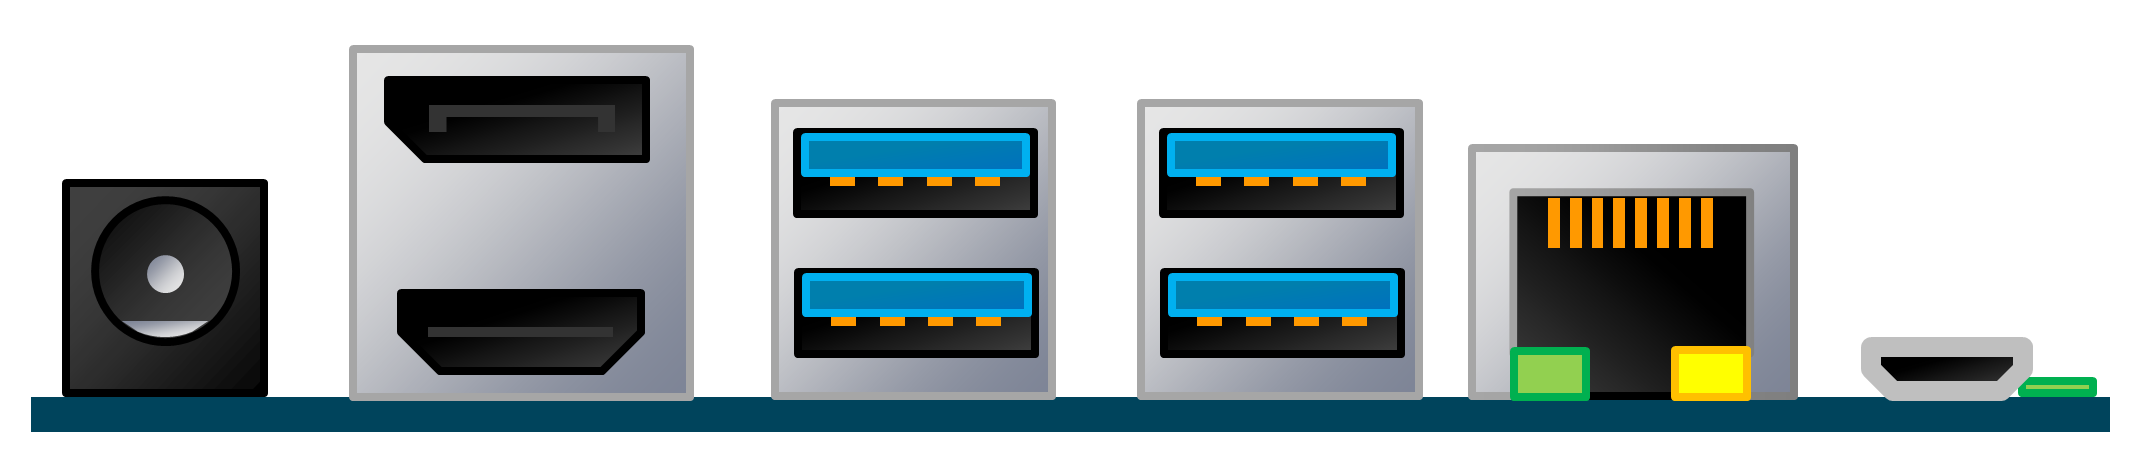
\includegraphics[scale=0.7]{Images/Jetson/JetsonNanoSide}};

\begin{figure}

\begin{tikzpicture}
  % Platine
  \draw[greenblue,fill=greenblue] (0,-0.02) -- (12.35,-0.02) -- (12.35,-0.2) -- (0,-0.2) -- cycle;
  
  % 5V 
  \pgfmathsetmacro{\xmin}{0.2};
  \pgfmathsetmacro{\xmax}{1.4};
  \pgfmathsetmacro{\ymin}{0};
  \pgfmathsetmacro{\ymax}{1.33};
  \draw[black,  fill=grayleft!30!grayright, postaction={path fading=west,  fill=grayleft},  line width=1.0pt] 
       (\xmin, \ymin) -- (\xmin, \ymax) -- (\xmax,\ymax) -- (\xmax, \ymin) -- cycle;

  \draw[silver,fill=silver,domain=0:360] plot ({0.8+0.11*cos(\x)}, {0.75+0.11*sin(\x)});
  \draw[silver,fill=silver,domain=230:310] plot ({0.8+0.4*cos(\x)}, {0.75+0.4*sin(\x)});
  \draw[black,line width=1.0pt,domain=0:360] plot ({0.8+0.4*cos(\x)}, {0.75+0.4*sin(\x)});

  %Display Port und HDMI
  \pgfmathsetmacro{\xmin}{1.9};
  \pgfmathsetmacro{\xmax}{3.95};
  \pgfmathsetmacro{\ymin}{0};
  \pgfmathsetmacro{\ymax}{2.1};
  \draw[graycircle!50, fill=white!20!graylight, postaction={path fading=west,  fill=grayright!60}, line width=1.0pt
  ] (\xmin, \ymin) -- (\xmin, \ymax) -- (\xmax,\ymax) -- (\xmax, \ymin) -- cycle;
  
  \draw[black,fill=grayleft!30!grayright, postaction={path fading=west,  fill=grayleft},
  line width=1.0pt]   (2.4, 0.17) -- (2.17,0.41) -- (2.17,0.64) -- (3.65,0.64) -- (3.65,0.41) -- (3.42,0.17) -- cycle;
  
  \pgfmathsetmacro{\xmin}{2.35};
  \pgfmathsetmacro{\xmax}{3.48};
  \pgfmathsetmacro{\ymin}{0.39};
  \pgfmathsetmacro{\ymax}{0.42};
  \draw[grayright,fill=grayright %graycircle!50, fill=white!20!graylight, postaction={path fading=west,  fill=grayright!60}, line width=1.0pt
  ] (\xmin, \ymin) -- (\xmin, \ymax) -- (\xmax,\ymax) -- (\xmax, \ymin) -- cycle;
  
  \draw[black,fill=grayleft!30!grayright, postaction={path fading=west,  fill=grayleft},
  line width=1.0pt] (2.33,1.42) -- (2.1, 1.65) -- (2.1,1.92) -- (3.66,1.92) -- (3.66,1.42) -- cycle;
  \draw[grayright,fill=grayright] (2.47, 1.7) -- (2.47,1.6) -- (2.37, 1.6) -- (2.37,1.75) -- (3.47,1.75) -- (3.47,1.6) -- (3.37,1.6) -- (3.37,1.7) -- cycle;
  
  % USV 3.0 - 2 x 2 
  \foreach \j in {0,...,1}
  {
	\pgfmathsetmacro{\xmin}{4.4+2.15*\j};
	\pgfmathsetmacro{\xmax}{6.1+2.15*\j};
	\pgfmathsetmacro{\ymin}{0};
	\pgfmathsetmacro{\ymax}{1.8};
	\draw[graycircle!50, fill=white!20!graylight, postaction={path fading=west,  fill=grayright!60}, line width=1.0pt] (\xmin, \ymin) -- (\xmin, \ymax) -- (\xmax,\ymax) -- (\xmax, \ymin) -- cycle;
	
	\foreach \i in {0,...,1}
	{
		\pgfmathsetmacro{\xmin}{4.54+2.16*\j};
		\pgfmathsetmacro{\xmax}{5.96+2.16*\j};
		\pgfmathsetmacro{\ymin}{0.27+0.86*\i};
		\pgfmathsetmacro{\ymax}{0.78+0.86*\i};
		\draw[black,fill=grayleft!30!grayright, postaction={path fading=west,  fill=grayleft},
		line width=1.0pt] 
		(\xmin, \ymin) -- (\xmin, \ymax) -- (\xmax,\ymax) -- (\xmax, \ymin) -- cycle;
		
		\pgfmathsetmacro{\xmin}{4.6+2.16*\j};
		\pgfmathsetmacro{\xmax}{5.91+2.16*\j};
		\pgfmathsetmacro{\ymin}{0.52+0.82*\i};
		\pgfmathsetmacro{\ymax}{0.73+0.82*\i};
		\draw[cyan, fill=deepskyblue, line width=1.0pt] 
		     (\xmin, \ymin) -- (\xmin, \ymax) -- (\xmax,\ymax) -- (\xmax, \ymin) -- cycle;
		
		\foreach \k in {0,...,3}
		{
			\pgfmathsetmacro{\xmin}{4.75+2.16*\j+0.29*\k};
			\pgfmathsetmacro{\xmax}{4.88+2.16*\j+0.29*\k};
			\pgfmathsetmacro{\ymin}{0.44+0.83*\i};
			\pgfmathsetmacro{\ymax}{0.48+0.83*\i};
			\draw[copper,fill=copper] (\xmin, \ymin) -- (\xmin, \ymax) -- (\xmax,\ymax) -- (\xmax, \ymin) -- cycle;
		}     
	}
  }
  
  % Ethernet
  \pgfmathsetmacro{\xmin}{8.55};
  \pgfmathsetmacro{\xmax}{10.5};
  \pgfmathsetmacro{\ymin}{0};
  \pgfmathsetmacro{\ymax}{1.5};
  \draw[graycircle!50, fill=white!20!graylight, postaction={path fading=west,  fill=grayright!60}, line width=1.0pt] (\xmin, \ymin) -- (\xmin, \ymax) -- (\xmax,\ymax) -- (\xmax, \ymin) -- cycle;

  \pgfmathsetmacro{\xmin}{8.8};
  \pgfmathsetmacro{\xmax}{10.2};
  \pgfmathsetmacro{\ymin}{0};
  \pgfmathsetmacro{\ymax}{1.25};
  \draw[black,  fill=grayleft!30!grayright, postaction={path fading=west,  fill=grayleft},  line width=1.0pt] (\xmin, \ymin) -- (\xmin, \ymax) -- (\xmax,\ymax) -- (\xmax, \ymin) -- cycle;

  \pgfmathsetmacro{\xmin}{8.8};
  \pgfmathsetmacro{\xmax}{9.25};
  \pgfmathsetmacro{\ymin}{0};
  \pgfmathsetmacro{\ymax}{0.3};
  \draw[darkpastelgreen,fill=greenyellow, line width=1.0pt] (\xmin, \ymin) -- (\xmin, \ymax) -- (\xmax,\ymax) -- (\xmax, \ymin) -- cycle;

  \pgfmathsetmacro{\xmin}{9.75};
  \pgfmathsetmacro{\xmax}{10.2};
  \pgfmathsetmacro{\ymin}{0};
  \pgfmathsetmacro{\ymax}{0.3};
  \draw[orange, fill=yellow, line width=1.0pt
  ] (\xmin, \ymin) -- (\xmin, \ymax) -- (\xmax,\ymax) -- (\xmax, \ymin) -- cycle;

  \foreach \j in {0,...,7}
  {
	\pgfmathsetmacro{\xmin}{9     + 0.13*\j};
	\pgfmathsetmacro{\xmax}{9.068 + 0.13*\j};
	\pgfmathsetmacro{\ymin}{0.92};
	\pgfmathsetmacro{\ymax}{1.25};
	\draw[copper,fill=copper]   (\xmin, \ymin) -- (\xmin, \ymax) -- (\xmax,\ymax) -- (\xmax, \ymin) -- cycle;
  }
  
  \pgfmathsetmacro{\xmin}{11.8};
  \pgfmathsetmacro{\xmax}{12.25};
  \pgfmathsetmacro{\ymin}{0};
  \pgfmathsetmacro{\ymax}{0.1};
  \draw[darkpastelgreen,fill=greenyellow, line width=1.0pt] (\xmin, \ymin) -- (\xmin, \ymax) -- (\xmax,\ymax) -- (\xmax, \ymin) -- cycle;
  
  % HDMI
  \draw[silver,fill=silver, line width=1.0pt] (11.0, 0) -- (11.7,0) -- (11.9,0.17) -- (11.9, 0.35) -- (10.8,0.35) --  (10.8, 0.17) -- cycle;
  
  \draw[black,fill=black] (11.05, 0.125) -- (11.65,0.125) -- (11.75,0.22) -- (11.75, 0.25) -- (10.95,0.25) --  (10.95, 0.22) -- cycle;
  
  \node (P1) at (0.8,-0.6) {5V DC};
  \node (P2) at (3,-0.8) {\begin{tabular}{c} Display Port \\ HDMI \end{tabular}};
  \node (P2) at (5.2,-0.8) {\begin{tabular}{c} USB 3.0 \\ USB 3.0 \end{tabular}};
  \node (P2) at (7.4,-0.8) {\begin{tabular}{c} USB 3.0 \\ USB 3.0 \end{tabular}};
  \node (P2) at (9.5,-0.6) { GigEth };
  \node (P2) at (11.8,-1) {\begin{tabular}{c} Micro USB\\ PWR oder \\ USB Device\end{tabular}};
  \node (P2) at (12.9,-1.8) {PWR LED};
  
\end{tikzpicture}
  \caption{Seitenansicht des Jetson Nanos} \label{JetonSeite}
\end{figure}	


\section{J41 Expansion Header Pinout}


%Pi-Enthusiasten werden die Ähnlichkeit in der Pin-Benennung bemerken. Ich habe die Pins nach Farben gruppiert, aber ich weiß immer noch nicht, was all die sekundären Funktionen der Pins sind. 
%Die Linux(BCM)-Spalte enthält zwei Zahlen. Die Zahlen in Klammern sind Raspberry-Pi-ähnliche GPIO-Nummern, so dass die gleichen GPIO-Bibliotheken wie die Raspberry-Pi verwendet werden können. 
%Diese Tabelle wird aktualisiert, nachdem NVIDIA weitere Dokumentation veröffentlicht hat (ich glaube, es wird in einigen Wochen erwartet). 

%\GRAPHICSC{1.0}{1.0}{Images/Jetson/JetsonNanoPins}
%\GRAPHICSC{0.7}{1.0}{Images/Jetson/gpio-pinout}





\newcommand{\GND}{\cellcolor{black}\textcolor{white}{GND}}
\newcommand{\Vf}{\cellcolor{red}\textcolor{black}{5V}}
\newcommand{\Vd}{\cellcolor{red}\textcolor{black}{3.3V}}
\definecolor{LightCyan}{rgb}{0.88,1,1}

\newcolumntype{a}{>{\columncolor{LightCyan}}c}

%{\scriptsize
%	\begin{tabular}{|p{20mm}|p{15mm}|p{15mm}|>{\columncolor{blue}}c|>{\columncolor{blue}}c|p{15mm}|p{15mm}|p{15mm}|} % >{\columncolor{green}}	% 
%		Alt Function & Linux (BCM) & Name & Pin & Pin & Name & Linux (BCM) & Alt Function \\ \hline
%		\cellcolor{orange} DAP4\_DOUT & 78(21) & D21 & 40 & 39 &\GND & & \\
%		\cellcolor{orange} DAP4\_DIN  & 77(20) & D20 & 38 & 37 & D26 & 12(26) & SPI2\_MOSI \\
%		UART2\_CTS   & 51(16) &       D16 & 36 & 35 & D19        & 76(19) & DAP4\_FS \\
%		&        &      \GND & 34 & 33 & D13        & 38(13) & GPIO\_PE6 \\
%		LCD\_BL\_PWM & 168(12)&       D12 & 32 & 31 & D6         & 200(6) & GPIO\_PZ0 \\
%		&        &      \GND & 30 & 29 & D5         & 149(5) & CAM\_AF\_EN \\
%		&        & D1/ID\_SC & 28 & 27 & D0/ID\_SD  &        & \\         
%		SPI1\_CS1    & 20(7)  &        D7 & 26 & 25 &\GND        &        &  \\
%		SPI1\_CS0    & 19(8)  &        D8 & 24 & 23 & D11        & 18(11) & SP1\_SCK \\
%		SPI2\_MISO   & 13(25) &       D25 & 22 & 21 & D9         & 17(9)  & SP1\_MISO \\
%		&        &      \GND & 20 & 19 & D10        & 16(10) & SP1\_MOSI \\
%		SPI2\_CS0    & 15(24) &       D24 & 18 & 17 & 3.3V       &        & \\   
%		SPI2\_CS1    & 232(23)&       D23 & 16 & 15 & D22        & 194(22)& LCD\_TE \\   
%		&        &      \GND & 14 & 13 & D27        & 14(27) & SPI2\_SCK \\
%		DAP4\_SCLK   & 79(18) &       D18 & 12 & 11 & D17        & 50(17) & UART2\_RTS \\
%		&        & RXD/D15   & 10 &  9 &\GND        &        & \\
%		&        & TXD/D14   &  8 &  7 & D4         & 216(4) & AUDIO\_MCLK\\
%		&        &\GND       &  6 &  5 & SCL/D3     &        & \\
%		&        & 5V        &  4 &  3 & SDA/D2     &        & \\
%		&        & 5V        &  2 &  1 & 3.3V       &        & \\
%	\end{tabular}
%}
%


\begin{table}
	
	\centering	
	{\small%\scriptsize
		\begin{tabular}{|c|c|a|a|c|c|} \hline
			\rowcolor{white}	 Sysfs GPIO &   \begin{tabular}{c} \textcolor{white}{I}\\ \textcolor{white}{I}\end{tabular}    Name   \begin{tabular}{c} \textcolor{white}{I}\\ \textcolor{white}{I}\end{tabular}     & Pin & Pin & Name & Sysfs GPIO  \\ \hline
			gpio78 & \begin{tabular}{c}I2S\_4\_SDOUT \\ D21 \\ \end{tabular}  & 40 & 39 & \GND   &  \\ \hline
			gpio77 & \begin{tabular}{c}I2S\_4\_SDIN  \\ D20 \\ \end{tabular}  & 38 & 37 & \begin{tabular}{c}SPI\_2\_MOSI  \\ D26 \\ \end{tabular}  & gpio12  \\ \hline
			gpio51 & \begin{tabular}{c}UART\_2\_CTS  \\ D16 \\ \end{tabular}  & 36 & 35 & \begin{tabular}{c}I2S\_4\_LRCK  \\ D19 \\ \end{tabular}  & gpio76  \\ \hline
			& \GND                                                     & 34 & 33 & \begin{tabular}{c}GPIO\_PE6  \\ D13 \\ \end{tabular}     & gpio38  \\ \hline
			gpio168& \begin{tabular}{c}LCD\_BL\_PWM \\ D12 \\ \end{tabular}   & 32 & 31 & \begin{tabular}{c}GPIO\_PZ0  \\ D6 \\ \end{tabular}      & gpio200  \\ \hline
			& \GND                                                     & 30 & 29 & \begin{tabular}{c}CAM\_AF\_EN  \\ D5 \\ \end{tabular}    & gpio149  \\ \hline
			&\begin{tabular}{c}I2C\_1\_SCL\\D1/I2C Bus 0\\\end{tabular} & 28 & 27 & \begin{tabular}{c}I2C\_1\_SDA\\ D0/I2C Bus 0\\\end{tabular}  &         \\   \hline     
			gpio20 & \begin{tabular}{c}SPI\_1\_CS1\\ D7\\\end{tabular}    & 26 & 25 &\GND        &          \\ \hline
			gpio19 & \begin{tabular}{c}SPI\_1\_CS0\\ D8\\\end{tabular}    & 24 & 23 & \begin{tabular}{c}SPI\_1\_SCK\\ D11\\\end{tabular}            & gpio18  \\ \hline
			gpio13 & \begin{tabular}{c}SPI\_2\_MISO\\ D25\\\end{tabular}  & 22 & 21 & \begin{tabular}{c}SPI\_1\_MISO\\ D9\\\end{tabular}            & gpio17   \\  \hline
			&      \GND                                            & 20 & 19 & \begin{tabular}{c}SPI\_1\_MOSI\\ D10\\\end{tabular}           & gpio16  \\ \hline
			gpio15 & \begin{tabular}{c}SPI\_2\_CS0\\ D24\\\end{tabular}   & 18 & 17 & \Vd        &         \\  \hline 
			gpio232& \begin{tabular}{c}SPI\_2\_CS1\\ D23\\\end{tabular}   & 16 & 15 & \begin{tabular}{c}LCD\_TE\\ D22\\\end{tabular}       & gpio194 \\   \hline
			&      \GND                                            & 14 & 13 & \begin{tabular}{c}SPI\_2\_SCK\\ D27\\\end{tabular}   & gpio14  \\ \hline
			gpio79 & \begin{tabular}{c}I2S\_4\_SCLK\\ D18\\\end{tabular}  & 12 & 11 & \begin{tabular}{c}UART\_2\_RTS\\ D17\\\end{tabular}  & gpio50  \\ \hline
			& \begin{tabular}{c}UART\_2\_RX\\ /dev/ttyTHS1 - D15\\\end{tabular}  & 10 &  9 &\GND        &         \\ \hline
			& \begin{tabular}{c}UART\_2\_TX\\ /dev/ttyTHS1 - D14\\\end{tabular}  &  8 &  7 & \begin{tabular}{c}AUDIO\_MCLK\\ D4\\\end{tabular}        & gpio216 \\ \hline
			&\GND       &  6 &  5 & \begin{tabular}{c}I2C\_2\_SCL\\ I2C Bus 1 - D3\\\end{tabular}     &         \\ \hline
			& \Vf       &  4 &  3 & \begin{tabular}{c}I2C\_2\_SDA\\ I2C Bus 1 - D2\\\end{tabular}     &         \\ \hline
			& \Vf       &  2 &  1 & \Vd        &     \begin{tabular}{c} \textcolor{white}{I}\\ \textcolor{white}{I}\end{tabular}              \\ \hline
		\end{tabular}
	}
	
	\caption{Pinbelegung der GPIOs des Jetson Nanos} \label{JetsonPins}
\end{table}


\begin{figure}
	
\begin{tikzpicture}[scale=1.4]
  % J40 Buttons
  \pgfmathsetmacro{\xmin}{0.17};
  \pgfmathsetmacro{\xmax}{0.82};
  \pgfmathsetmacro{\ymin}{7.7};
  \pgfmathsetmacro{\ymax}{9};
  \draw[darkcyan,fill=greenblue,
     line width=1.6pt] (\xmin, \ymin) -- (\xmin, \ymax) -- (\xmax,\ymax) -- (\xmax, \ymin) -- cycle;

  \foreach \j in {0,...,1}
  {
	\foreach \i in {0,...,3}
	{
		\pgfmathsetmacro{\d}{0.05}
		\pgfmathsetmacro{\x}{0.35+0.312*\j};
		\pgfmathsetmacro{\y}{7.87+0.312*\i};
		\draw[yellow,fill=yellow] ({\x-\d}, {\y-\d} ) -- ({\x+\d}, {\y-\d}) -- ({\x+\d}, {\y+\d}) -- ({\x-\d}, {\y+\d}) -- cycle;
	}
  }
  \pgfmathsetmacro{\d}{0.05}
  \pgfmathsetmacro{\x}{0.35+0.312};
  \pgfmathsetmacro{\y}{7.87+0.312*0};
  \draw[yellow,thick,fill=fuchsia] ({\x-\d}, {\y-\d} ) -- ({\x+\d}, {\y-\d}) -- ({\x+\d}, {\y+\d}) -- ({\x-\d}, {\y+\d}) -- cycle;
  
  \node[right]  (P4) at (1,8.85) {DIS (disable auto power-on)};
  \node[right]  (P3) at (1,8.5) {RST (system reset)};
  \node[right]  (P2) at (1,8.15) {DIS (FRC (board recovery mode))};
  \node[right]  (P1) at (1,7.8) {DIS (ON (power on) )};

\end{tikzpicture}

  \caption{J40 Buttons}
\end{figure}  

\begin{figure}
\begin{tikzpicture}[scale=1.4]
  %J44 Serial
  \pgfmathsetmacro{\xmin}{1.2};
  \pgfmathsetmacro{\xmax}{1.5};
  \pgfmathsetmacro{\ymin}{8.02};
  \pgfmathsetmacro{\ymax}{9.95};
  \draw[darkcyan,fill=greenblue,
        line width=1.6pt] (\xmin, \ymin) -- (\xmin, \ymax) -- (\xmax,\ymax) -- (\xmax, \ymin) -- cycle;

  \foreach \j in {0,...,0}
  {
	\foreach \i in {0,...,5}
	{
		\pgfmathsetmacro{\d}{0.05}
		\pgfmathsetmacro{\x}{1.35+0.312*\j};
		\pgfmathsetmacro{\y}{8.2+0.312*\i};
		\draw[yellow,fill=yellow] ({\x-\d}, {\y-\d} ) -- ({\x+\d}, {\y-\d}) -- ({\x+\d}, {\y+\d}) -- ({\x-\d}, {\y+\d}) -- cycle;
	}
  }
  \pgfmathsetmacro{\d}{0.05}
  \pgfmathsetmacro{\x}{1.35};
  \pgfmathsetmacro{\y}{8.2+0.312*0};
  \draw[yellow,thick,fill=fuchsia] ({\x-\d}, {\y-\d} ) -- ({\x+\d}, {\y-\d}) -- ({\x+\d}, {\y+\d}) -- ({\x-\d}, {\y+\d}) -- cycle;
  
  \node[right]  (P5) at (1.7,9.81) {CTS};
  \node[right]  (P5) at (1.7,9.48) {TXD};
  \node[right]  (P4) at (1.7,9.16) {TXD};
  \node[right]  (P3) at (1.7,8.82) {N/A};
  \node[right]  (P2) at (1.7,8.51) {RTS};
  \node[right]  (P1) at (1.7,8.16) {GND};
\end{tikzpicture}

\caption{J44 Serielle Schnittstelle - 3.3V 115200 Baud, 8N1} 
\end{figure}

\begin{figure}
  \begin{tikzpicture}[scale=1.4]
  % J15 5V Fan
  \pgfmathsetmacro{\xmin}{9.33};
  \pgfmathsetmacro{\xmax}{10.55};
  \pgfmathsetmacro{\ymin}{2.86};
  \pgfmathsetmacro{\ymax}{3.55};
  \draw[darkcyan,fill=greenblue,  line width=1.6pt] 
       (\xmin, \ymin) -- (\xmin, \ymax) -- (\xmax,\ymax) -- (\xmax, \ymin) -- cycle;

  \pgfmathsetmacro{\xmin}{9.8};
  \pgfmathsetmacro{\xmax}{10.45};
  \pgfmathsetmacro{\ymin}{3.35};
  \pgfmathsetmacro{\ymax}{3.55};
  \draw[darkcyan,
        line width=1.6pt] (\xmin, \ymin) -- (\xmin, \ymax) -- (\xmax,\ymax) -- (\xmax, \ymin) -- cycle;

  \foreach \j in {0,...,3}
  {
	\foreach \i in {0,...,0}
	{
		\pgfmathsetmacro{\d}{0.05}
		\pgfmathsetmacro{\x}{9.45+0.317*\j};
		\pgfmathsetmacro{\y}{3.18 +0.323*\i};
		\draw[blue,fill=yellow] ({\x-\d}, {\y-\d} ) -- ({\x+\d}, {\y-\d}) -- ({\x+\d}, {\y+\d}) -- ({\x-\d}, {\y+\d}) -- cycle;
	}
  }

  \draw[dotted] (9.45, 3.18) -- (9.45, 4.85) -- (9.6, 4.85);
  \node[right]  (P4) at (9.6,4.85) {GND};
  \draw[dotted] (9.45+0.317, 3.18) -- (9.45+0.317, 4.5) -- (9.6+0.317, 4.5);
  \node[right]  (P3) at (9.6+0.317,4.5) {5V};
  \draw[dotted] (9.45+0.317+0.317, 3.18) -- (9.45+0.317+0.317, 4.15) -- (9.6+0.317+0.317, 4.15);
  \node[right]  (P2) at (9.6+0.317+0.317,4.15) {TACH};
  \draw[dotted] (9.45+0.317+0.317+0.317, 3.18) -- (9.45+0.317+0.317+0.317, 3.8) -- (9.6+0.317+0.317+0.317, 3.8);
  \node[right]  (P1) at (9.6+0.317+0.317+0.317,3.8) {PWM};

  \end{tikzpicture}

  \caption{J15 5V-Lüfter} 
\end{figure}




\subsection{Technische Daten}

\begin{tabular}{ll}
	GPU  &  NVIDIA-Grafikprozessor mit der Maxwell\textsuperscript{\texttrademark}-Architektur und 128 \\
	&   NVIDIA CUDA\textsuperscript{\textregistered}-Recheneinheiten \\
	CPU  &  Quad-Core-Prozessor ARM\textsuperscript{\textregistered} Cortex\textsuperscript{\textregistered}-A57 MPCore processor \\
	Arbeitsspeicher &   4 GB 64-bit LPDDR4 \\
	Datenspeicher  &  16 GB eMMC 5.1-Flashspeicher \\
	Videokodierung  &  4K bei 30 (H.264/H.265) \\
	Videodekodierung &   4K bei 60 (H.264/H.265) \\
	Kamera  &  12 Spuren (3x4 oder 4x2) MIPI CSI-2 DPHY 1.1 (1,5 Gbit/s) \\
	Anschlüsse  &  Gigabit-Ethernet \\
	Bildschirme  &  HDMI 2.0 oder DP1.2 | eDP 1.4 | DSI (1 x2) 2 simultan \\
	UPHY  &  1 $\times$ 1/2/4 PCIE, 1 $\times$ USB 3.0, 3 $\times$ USB 2.0 \\
	Anschlüsse &   1 $\times$ 1/2/4 PCIE, 1 $\times$ USB 3.0, 3$\times$ USB 2.0 \\
	Größe  &  69,6 mm $\times$ 45 mm \\
	Mechanik  &  260-poliger Randstecker  \\
\end{tabular}


